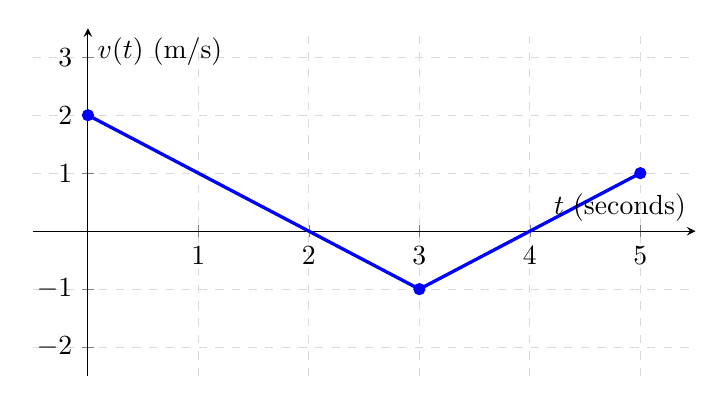
\begin{tikzpicture}
\begin{axis}[
    axis lines=middle,
    xlabel={$t$ (seconds)},
    ylabel={$v(t)$ (m/s)},
    xmin=-0.5, xmax=5.5,
    ymin=-2.5, ymax=3.5,
    xtick={0,1,2,3,4,5},
    ytick={-2,-1,0,1,2,3},
    width=10cm,
    height=6cm,
    grid=major,
    grid style={dashed,gray!30}
]

% Piecewise linear: starts at v=2, drops to v=-1 at t=3, then rises to v=1 at t=5
\addplot[blue, very thick] coordinates {(0,2) (3,-1) (5,1)};

% Mark key points
\addplot[only marks, mark=*, mark size=2pt, blue] coordinates {(0,2) (3,-1) (5,1)};

\end{axis}
\end{tikzpicture}